% !TeX program = lualatex
% !TeX encoding = utf8
% !TeX spellcheck = uk_UA
% !TeX root =../FTProblems.tex

%=========================================================
\Opensolutionfile{answer}[\currfilebase/\currfilebase-Answers]
\Writetofile{answer}{\protect\section*{\nameref*{\currfilebase}}}
\chapter{Електро- та магнітостатика у вакуумі}\label{\currfilebase}
%=========================================================
%\epigraph{\Annabelle  ...взаимное притяжение электрической жидкости, именуемой положительной, и электрической жидкости, именуемой обычно отрицательной, состоит в обратном отношении квадратов расстояний...
%}{Шарль Огюстен Кулон}

\section{Прості задачі на рівняння Максвелла}

%=========================================================
\begin{problem}\label{prb:potter}
Заряд $q$ розташований на верхній основі горщика (там, де мала бути кришка) на деякій відстані від осі (рис.~\ref{pic:potter}). Знайти потік
вектора
напруженості електричного поля, створюваного зарядом, через бічні стінки та дно горщика. Відстань заряду до осі, параметри, що визначають
форму та
розміри горщика задайте самостійно.
\end{problem}

%=========================================================
\begin{problem}\label{prb:tube}
Труба має довжину $10$~м та діаметр $5$~см. Заряд $q$ розташований на вході в трубу з лівого кінця (рис.~\ref{pic:tube}).
Знайти потік вектора напруженості електричного поля, створюваного зарядом, через стінки труби з точністю до другого знаку після коми.
\end{problem}

%=========================================================
\begin{figure}[h!]\centering
%---------------------------------------------------------
\begin{minipage}[t]{0.45\linewidth}\centering
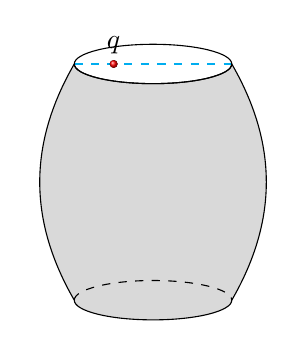
\begin{tikzpicture}[]
    \draw[fill=gray!30] (-1, 3) to[bend right] (-1, 0) arc(180:360:1 and 0.25) to[bend right] (+1, 3) arc(0:-180:1 and 0.25);
    \draw[dashed, cyan] (-1, 3) -- (+1, 3);
%    \draw (+1, 3) to[bend left] (+1, 0);
%    \draw (0, 0) circle (1 and 0.25);
    \draw (0, 3) circle (1 and 0.25);
    \draw[dashed] (-1, 0) arc(180:0:1 and 0.25);
     \fill [ball color=red] (-0.5, 3) circle (0.05) node[above] {$q$};
\end{tikzpicture}
\caption{До задачі~\ref{prb:potter}}
\label{pic:potter}
\end{minipage}
%---------------------------------------------------------
\begin{minipage}[t]{0.45\linewidth}\centering
    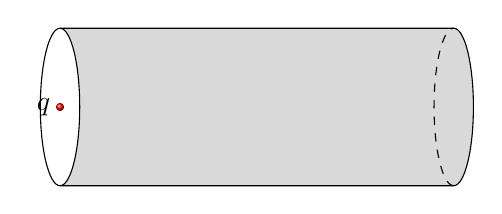
\begin{tikzpicture}
        \def\r{2}
        \draw [fill=gray!30] (0, {\r/2}) -- ++(5, 0) arc (90:-90:0.25 and {\r/2}) -- ++(-5, 0) arc (-90:+90:0.25 and {\r/2}) -- cycle;
        \draw (0, -{\r/2}) arc(270:90:0.25 and {\r/2});
        \draw[dashed] (5, -{\r/2}) arc(270:90:0.25 and {\r/2});
        \fill [ball color=red] (0, 0) circle (0.05) node[left] {$q$};
    \end{tikzpicture}
\caption{До задачі~\ref{prb:tube}}
\label{pic:tube}
\end{minipage}
%---------------------------------------------------------
\end{figure}
%=========================================================




%=========================================================
\begin{problem}\label{prb:intLB}
Струм $I$  тече у додатному напрямку осі $OZ$ декартових координат (рис.~\ref{pic:intB}).
Знайти інтеграл $\int\limits_L \Bfield(\vect{r})\cdot d\vect{r}$ по траєкторії $L$, що показано червоним кольором на рисунку;  $\Bfield$ ---
індукція
магнітного поля, створюваного струмом.
\end{problem}


%=========================================================
\begin{problem}\label{prb:flux_rotated_hemisphere}
Знайти потік індукції однорідного магнітного поля $\Bfield$ поверхню нахиленої напівкулі радіуса $R$ (рис.~\ref{pic:flux_rotated_hemisphere}). Вектор
$\Bfield$
спрямований  вертикально; площина основи нахилена на кут $\alpha$ до горизонтальної площини.
\end{problem}



%=========================================================
\begin{figure}[h!]\centering
%---------------------------------------------------------
\begin{minipage}[t]{0.45\linewidth}\centering
\begin{tikzpicture}[>=latex,
		midarrow/.style={
				postaction={ decorate,
						decoration={ markings, mark=at position .55 with {\arrow{>}}}}
			},
		sig/.style={font=\scriptsize, text=black},
	]
	\draw[->] (0,0) -- ++(2, 0) node[below] {$y$};
	\draw[->] (0,0) -- ++(225:1.75) node[below] {$x$};
	\draw[->] (0,0) -- ++(0, 2) node[left] {$z$};

	\draw[dashed] (0,0) -- ++(-2, 0);
	\draw[dashed] (0,0) -- ++(225:-1.75);
	\draw[dashed] (0,0) -- ++(0, -2);

	\draw[postaction={ decorate,
				decoration={ markings, mark=at position .7 with {\arrow{>}}}}, ultra thick, gray] (0, -1.75) -- node[pos=0.7, left] {$I$}
				(0, 1.75);
	\draw[red, thick, midarrow] (-1.5, 0) coordinate (-b) node[sig, above]  {$-b$} -- (-0.5, 0) coordinate (-a) node[sig, above]  {$-a$} --
	++(225:0.5)
	-- ++(1, 0) --
	++(225:-0.5) coordinate (a)
	node[sig, above]  {$a$}  -- ++(1, 0) coordinate (b) node[sig, above]  {$b$};

    \draw (-b) -- +(0,0.1) -- +(0, -0.1)
          (-a) -- +(0,0.1) -- +(0, -0.1)
          (a) -- +(0,0.1) -- +(0, -0.1)
          (b) -- +(0,0.1) -- +(0, -0.1);


    \draw[|-|] (0.65, 0) -- node[pos=0.5, sig, anchor=north west] {$h$} ++(225:0.5);
\end{tikzpicture}
\caption{До задачі~\ref{prb:intLB}}
\label{pic:intB}
\end{minipage}
%---------------------------------------------------------
\begin{minipage}[t]{0.45\linewidth}\centering
    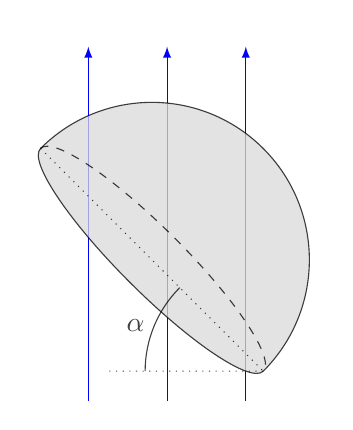
\begin{tikzpicture}[>=latex]
        \foreach[count=\c] \x in {0.9,...,3.6}{
            \draw[->, blue] (\x, -2.5) -- ++(0, 4.5)
            \ifnum\c=2
            node[above] {$\Bfield$}
            \fi
            ;
        }
        \begin{scope}[
            rotate around={-45:(1,0)},
            opacity=0.75]
            \draw[fill=gray!30] (0,0) arc (180:0:2) arc(0:-180:2 and {2*0.2});
        \draw[dashed] (0,0) arc (180:0:2 and {2*0.2});
        \draw[dotted] (0,0) -- (4,0);
        \draw[dotted] (4,0) -- ++(45:-2);
        \draw (4,0)  ++(-1.5,0) arc(180:{180+45}:1.5) node[pos=0.5, anchor=east] {$\alpha$};
        \end{scope}

    \end{tikzpicture}
\caption{До задачі~\ref{prb:flux_rotated_hemisphere}}
\label{pic:flux_rotated_hemisphere}
\end{minipage}
%---------------------------------------------------------
\end{figure}



%=========================================================
\begin{problem}\label{prb:charge_in_hole}
Усередині незарядженої металевої кулі якимось чином зробили сферичну порожнину (рис.~\ref{pic:charge_in_hole}), в центрі якої помістили
заряд  $q$.
Знайти напруженість електричного поля в усьому просторі.
\end{problem}

%=========================================================
\begin{problem}\label{prb:charge_in_elhole}
Усередині незарядженої металевої кулі якимось чином зробили порожнину у формі еліпсоїда (рис.~\ref{pic:charge_in_elhole}), в порожнину помістили
заряд  $q$ (не обов’язково в центрі).
Знайти напруженість електричного поля \emph{зовні} кулі.
\end{problem}

%=========================================================
\begin{figure}[h!]\centering
%---------------------------------------------------------
\begin{minipage}[t]{0.45\linewidth}\centering
		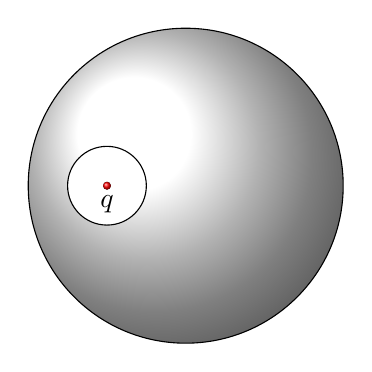
\begin{tikzpicture}
			\draw [ball color=white] (0,0) circle (2);
%			\draw [-stealth] (0,0) -- node[above left] {$R$} (60:2);
			\draw [fill=white] (-1,0) circle (0.5);
			\fill [ball color=red] (-1,0) circle (0.05) node[below] {$q$};
		\end{tikzpicture}
		\caption{До задачі~\ref{prb:charge_in_hole}}
		\label{pic:charge_in_hole}
\end{minipage}
%---------------------------------------------------------
\begin{minipage}[t]{0.45\linewidth}\centering
		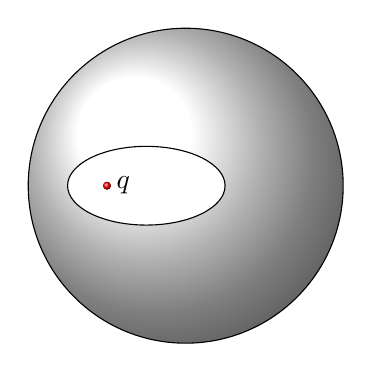
\begin{tikzpicture}
			\draw [ball color=white] (0,0) circle (2);
%			\draw [-stealth] (0,0) -- node[above left] {$R$} (60:2);
			\draw [fill=white] (-0.5,0) circle (1 and 0.5);
			\fill [ball color=red] (-1,0) circle (0.05) node[right] {$q$};
		\end{tikzpicture}
		\caption{До задачі~\ref{prb:charge_in_elhole}}
		\label{pic:charge_in_elhole}
\end{minipage}
%---------------------------------------------------------
\end{figure}




%=========================================================

\begin{problem}
Використовуючи $\delta$-функцію, запишіть вираз для об'ємної густини заряду у сферичній системі координат  для випадків:
\begin{enumerate}[label=\alph*)]
	\item точкового сферично-симетричного заряду $q$, що розташований у початку координат;
	\item заряду $q$, що рівномірно розподілений по кільцю радіусом $R$, що лежить в площині $XOY$;
	\item заряду, що розподілений по кільцю радіусом $R$ з лінійною густиною $\lambda(\phi)$, що лежить в площині $XOY$;
	\item заряду $q$, що розподілений рівномірно по сферичній  поверхні радіусу $R$;
	\item заряду, що розподілений по сферичній поверхні радіуса $R$ з поверхневою густиною $\sigma (\theta)$.
\end{enumerate}
\begin{solution}
	\begin{enumerate*}[label=\alph*)]
		\item $\rho = q\delta(\vect{r})$;
		\item $\rho = \frac{q}{2\pi R^2}\delta(r - R)\delta(\cos\theta)$;
		\item $\rho = \frac{\lambda(\phi)}{R}\delta(r - R)\delta(\cos\theta)$;
		\item $\rho = \frac{q}{4\pi R^2}\delta (r - R)$;
		\item $\rho = \sigma (\theta)\delta (r - R)$.
	\end{enumerate*}
\end{solution}
\end{problem}


%\subsection*{Електричне поле}

%=========================================================
\begin{problem}
Електричне поле утворене однорідним розподілом зарядів з густиною $\rho(r,\theta,\phi) = \rho_0$ усередині кулі радіуса $R$, зовні зарядів немає. Знайти модуль напруженості та потенціал електричного поля. Побудуйте графіки їх залежностей від $r$.
\end{problem}


%=========================================================
\begin{problem}
Електричне поле утворене розподілом зарядів $\rho = \rho_0\left( \frac{r}{R}\right)^n $   всередині кулі радіуса $R$, зовні зарядів немає. Знайти напруженість електричного поля та потенціал в усьому просторі.
\end{problem}

%\subsection*{Магнітне поле}

%=========================================================
\begin{problem}
Виходячи із закону Біо-Савара-Лапласа показати, що для замкнутого контуру зі струмом $I$ напруженість магнітного поля в деякій точці $P$ з координатами $(x,y,z)$ виражається формулою $\Bfield = \frac{I}{c} \vect{\nabla}\Omega$, де $\Omega$~--- тілесний кут, під яким контур видно з цієї точки.
\begin{solution}
    Тілесний кут, під яким видно поверхню $S$ з точки $r$:
    \[
        \Omega(\vect{r}) = \int\limits_S d\vect{S}'\frac{\vect{r}' - \vect{r}}{|\vect{r}' - \vect{r}|^3}.
    \]
    Обчислимо зміну тілесного кута при зсуві точки спостереження на малий вектор $\delta\vect{r}$   ($\vect{r} \to \vect{r} + \delta\vect{r}$, контур залишається нерухомим). Це можна зробити, залишаючи, навпаки, точку $\vect{r}$  нерухомою, але зсуваючи поверхню $S$  на $-\delta\vect{r}$, тобто у протилежному напрямку. При цьому зміна $\Omega$ відбувається за рахунок тонкої смужки, яка відповідає переміщенню контура $L$ , який є границею $S$ ($\delta d{\vect{S}} =  - \delta\vect{r} \times d{\vect{l}'}$):
    \[
        \delta\Omega(\vect{r}) = \delta\vect{r}\times \vect{\nabla}\Omega = -\oint \delta\vect{r}\times d\vect{l}' \cdot \frac{\vect{r}' - \vect{r}}{|\vect{r}' - \vect{r}|^3} = - \oint  d\vect{l}' \times \cdot \frac{\vect{r}' - \vect{r}}{|\vect{r}' - \vect{r}|^3} \delta\vect{r}.
    \]
    Звідси виходячи з властивості тілесного кута, під яким видно замкнений контур $L$:
	\[
		\vect{\nabla}\Omega = - \oint  d\vect{l}' \times \cdot \frac{\vect{r}' - \vect{r}}{|\vect{r}' - \vect{r}|^3} = \oint  d\vect{l}' \times  \frac{\vect{r} - \vect{r}'}{|\vect{r} - \vect{r}'|^3}.
	\]
    З іншого боку, індукція в точці $\vect{r}$, створювана струмом в контурі $L$, є
	\[
		\Bfield = \frac{I}{c} \oint  d\vect{l}' \times  \frac{\vect{r} - \vect{r}'}{|\vect{r} - \vect{r}'|^3} = \frac{I}{c} \vect{\nabla}\Omega.
	\]
\end{solution}
\end{problem}


%=========================================================
\begin{problem}
Знайти індукцію магнітного поля, якщо густина струму $\vect{j}_0 = j_0\vect{e}_y$   в області  $0 < z < a$ (декартові координати $x$, $y$, $z$). Зовні струмів немає.
\end{problem}

%=========================================================
\begin{problem}
Знайти індукцію магнітного поля площини $z=0$, якщо поверхнева густина струму $\vect{i}_0 = i_0\vect{e}_x$. Результат подати у векторному вигляді через орти декартової системи координат.
\end{problem}

%=========================================================
\begin{problem}
Знайти індукцію магнітного поля нескінченного прямого проводу зі струмом  $I_0$. Напрямок провідника заданий одиничним вектором $\vect{e}_0$. Результат подати у векторному вигляді через вектори $\vect{r} \perp \vect{e}_0$.
\end{problem}

%=========================================================
\begin{problem}
Струм $\vect{j} = j(r)\vect{e}_0$ протікає вздовж нескінченного циліндру радіуса $R$. Зовні струмів немає. Напрямок осі циліндра задається одиничним вектором $\vect{e}_0$. Знайти індукцію магнітного поля у всьому просторі. Результат подати у векторному вигляді через вектори $\vect{r} \perp \vect{e}_0$.
\begin{solution}
	$\vect{B}(r) = \frac{4\pi}{cr^2}\left[ \vect{e}_0 \times \vect{r} \right]\int\limits_0^r j(r)r dr$.
\end{solution}
\end{problem}

%=========================================================
\begin{problem}
Заряд рівномірно розподілений в області  $0 < z < a$. Зовні зарядів немає. Знайти напруженість електричного поля  у всьому простору.
\end{problem}

%=========================================================
\begin{problem}
Визначити величину та напрямок стаціонарного магнітного поля, утвореного струмом всередині нескінченного циліндричного провідника радіуса $R$, вісь якого збігаться з віссю аплікат.  Густина струму   $\vect{j}(r, \theta,\phi) = j_0\vect{e}_z \left( 1- \frac{r}{a}\right) $. Зовні струмів немає.
\end{problem}

%=========================================================
\begin{problem}
Електричне поле в усьому просторі має вигляд:
\[
	\Efield = \Efield_0 (\vect{a}\cdot \vect{r}),
\]
де $\Efield_0$ та $\vect{a}$~--- постійні вектори. Знайдіть густину зарядів, що створили дане поле.
\end{problem}

%=========================================================
\begin{problem}
В стаціонарній системі індукція магнітного поля дається виразом $\Bfield = \Bfield_0 (\vect{a}\cdot \vect{r})$, а $(\vect{a}\cdot \Bfield_0) = 0$.  Електричного поля немає. $\Bfield_0$ та $\vect{a}$~--- постійні вектори. Знайти густину струму, що створює дане поле.
\end{problem}

%=========================================================
\begin{problem}
В стаціонарній системі індукція магнітного поля дорівнює
\[
	\Bfield = \left[ \Bfield_0 - \vect{a}(\vect{a} \cdot \Bfield_0)\right]  (\vect{a}\cdot \vect{r}),
\]
$\vect{a}^2 = 1$, а $\Bfield_0$ та $\vect{a}$~--- постійні вектори. Знайти густину струму, що створює дане поле.
\end{problem}

\section{Рівняння Пуассона та Лапласа. Граничні задачі електростатики}

\begin{Theory}

	Зв'язок напруженості та потенціалу:
	\begin{equation}\label{E-phi}
		\Efield = - \vect{\nabla}\pot.
	\end{equation}
	З урахуванням~\eqref{E-phi}, з рівняння \eqref{Diff I}  отримуємо рівняння Пуассона:
	\begin{equation}\label{Poisson's_equation}
		\Delta\pot = -4\pi\rho.
	\end{equation}

	В областях, де заряди відсутні, рівняння~\eqref{Poisson's_equation} приймає вигляд рівнянням Лапласа:
	\begin{equation}\label{Laplace_equation}
		\Delta\pot = 0.
	\end{equation}

	Рівняння Пуассона само собою має безліч розв'язків. Для кусково-неперервного розподілу об’ємної густини заряду  $\rho(\vect{r})$, щоб визначити розв’язок єдиним чином в області $\Omega$ , можна задати значення $\pot(\vect{r})$  на границях цієї області. Якщо $\Omega$  необмежена, зазвичай накладають умову:
	\begin{equation}\label{eq:Efinity}
		\lim\limits_{r \to \infty } \left\{ {\left| {\nabla \pot({\vect{r}})} \right|{r^2}} \right\} < \infty ,\quad r = \left| {\vect{r}} \right|.
	\end{equation}

	Якщо область  $\Omega$ складається з двох частин, розділених поверхнею $\partial\Omega$, на якій є поверхневі заряди, слід додати граничні умови \eqref{EtauBc}, \eqref{EnBc} на $\partial\Omega$. Також можна замість \eqref{EtauBc} задати умову неперервності потенціалу при перетині $\partial\Omega$. За цих умов розв'язок~\eqref{Poisson's_equation} визначений єдиним чином.

	За наявності провідника, розташованого всередині замкненої поверхні $\partial\Omega$,  слід задавати значення потенціалу:
	\begin{equation}\label{eq:MetBound}
		\left. \pot  \right|_{\vect{r} \in \partial \Omega}  = \pot_0 \equiv \const
	\end{equation}
	на цій поверхні.

	Замість~ \eqref{eq:MetBound}, можна задати повний заряд на провіднику
	\begin{equation}\label{}
		q = -\frac{1}{4\pi}\int\limits_{\partial\Omega} dS (\vect{n}\cdot\vect{\nabla}\pot) =  -\frac{1}{4\pi}\int\limits_{\partial\Omega} dS \frac{\partial \pot}{\partial n},
	\end{equation}
    $\vect{n}$~---	зовнішня нормаль на поверхні провідника; при цьому вважаємо, що потенціал на поверхні $\left. \pot  \right|_{\vect{r} \in \partial \Omega}  = \const$, хоча значення цієї константи задавати не потрібно.


	Розв'язком рівнянь Пуассона у випадку ізольованої системи зарядів
	\begin{equation}\label{Supperposition_principle}
		\pot(\vect{r}) = \iiint\limits_{} \frac{\rho(\vect{r'}) dV'}{\left| \vect{r} - \vect{r'} \right|}.
	\end{equation}
	де $\vect{r}'$~--- радіус-вектор елемента заряду $\rho(\vect{r'}) dV'$, а $\vect{r}$~--- радіус-вектор точки спостереження.

Енергія електростатичного поля з потенціалом $\pot(\vect{r})$, створюваного об’ємними зарядами з густиною $\rho(\vect{r})$  та зарядами з поверхневою густиною $\sigma$  на межі розділу середовищ $S$:


\begin{equation}\label{eq:We}
W_e = \frac{1}{8\pi}\int {dV} \, \Efield^2(\vect{r}) = \frac{1}{2}\int\limits_\infty  dV\, \rho (\vect{r}) \pot(\vect{r}) + \frac{1}{2}\int\limits_S dS\, \sigma(\vect{r}) \phi (\vect{r}).
\end{equation}


	У задачах магнітостатики маємо справу з рівняннями
	\begin{equation}\label{eq:Bstatic}
		\divg\Bfield = 0, \quad \rot\Bfield = \frac{4\pi}{c}\vect{j}.
	\end{equation}

	Для ізольованої системи струмів, за умови спадання на нескінченності
	\begin{equation}\label{}
		\lim\limits_{r \to \infty } \left\{ {\left| \Bfield(\vect{r}) \right|{r^2}} \right\} < \infty ,\quad r = \left| {\bf{r}} \right|,
	\end{equation}
	аналогічно~\eqref{eq:Efinity}, та з граничними умовами \eqref{BtauBc}, \eqref{BnBc}~--- за наявності поверхневих струмів, можна показати, що розв’язок рівнянь~\eqref{eq:Bstatic} визначений єдиним чином.

	Для вектор-потенціалу з використанням калібрувальної умови $\vect\nabla\cdot\vect{A} = 0$ (кулонівське калібрування) отримуємо рівняння:
	\begin{equation}
		\nabla^2\vect{A} = - \frac{4\pi}{c}\vect{j},
	\end{equation}
    розв'язком цього рівняння для ізольованої системи струмів є
	\begin{equation}
		\vect{A} = \frac1c \iiint\limits_{} \frac{\vect{j'}(\vect{r}') dV'}{\left| \vect{r} - \vect{r'} \right|},
	\end{equation}
	де $\vect{r}'$~--- радіус-вектор елемента струму $\vect{j'}(\vect{r}') dV'$, а $\vect{r}$~--- радіус-вектор точки спостереження.

Енергія магнітостатичного поля з вектор-потенціалом $\vect{A}$, створюваного об’ємними струмами з густиною $\vect{j}$ та струмами з поверхневою  густиною $\vect{i}$  на межі розділу середовищ $S$:
\begin{equation}\label{eq:Wm}
    W_m = \frac{1}{{8\pi }}\int dV \,\Bfield^2(\vect{r}) = \frac{1}{2}\int dV \, \vect{j}(\vect{r}) \cdot \vect{A}(\vect{r}) + \frac{1}{2}\int {dS} \, \vect{i}(\vect{r}) \cdot \vect{A}(\vect{r}).
\end{equation}

    \bigskip

	Розкладання розв'язків рівняння Лапласа~\eqref{Laplace_equation} в ряд по ортогональній системі функцій --- один з найбільш ефективних методів вирішення широкого класу задач. Конкретний вибір ортогональної системи функцій залежить від симетрії, яку має (точно або наближено) система, що розглядається.

	\bigskip\textit{Декартові координати}. Рівняння Лапласа в декартових координатах має вигляд:
	\begin{equation}\label{eq:Laplase_eqn_Cartesian}
		\frac{\partial^2\pot}{\partial x} + \frac{\partial^2\pot}{\partial y} + \frac{\partial^2\pot}{\partial z} = 0.
	\end{equation}
	За певних умов розв'язок цього рівняння можна представити у вигляді як добутку трьох функцій, кожна з яких залежить лише від однієї координати:
	\begin{equation*}
		\pot = X(x)Y(y)Z(z).
	\end{equation*}

	У більш загальному випадку розв'язок рівняння Лапласа подають як суму подібних добутків.


	\bigskip\textit{Сферичні координати}. Для випадку задач з азимутальною симетрією розв'язком рівняння~\eqref{Laplace_equation} є вираз:
	\begin{equation}\label{eq:Laplase_Azimuthal}
		\pot(r, \theta) =  \sum\limits_{l = 0}^{\infty} \left(A_l \left( \frac{r}{R}\right)^l + B_l \left( \frac{r}{R}\right)^{-(l+1)} \right) P_l(\cos\theta) ,
	\end{equation}
	де коефіцієнти $A_l$ та $B_l$ визначаються з граничних умов, $P_l(\cos\theta)$~--- поліноми Лежандра (див. додаток~\ref{Polinoms}).

	\bigskip\textit{Циліндричні координати}. У випадку циліндричної симетрії, розв'язком рівняння~\eqref{Laplace_equation} є вираз:
	\begin{multline}\label{eq:Laplase_Cylindrical}
		\pot(r, \phi) =  A_0 + B_0 \ln r + \\ +\sum\limits_{m = 1}^{\infty} \left[\left(A_m\left( \frac{r}{R}\right)^m + B_m\left( \frac{R}{r}\right)^m\right)\sin m\phi + \left(C_m\left( \frac{r}{R}\right)^m + D_m\left( \frac{R}{r}\right)^m\right)\cos{m\phi} \right],
	\end{multline}
	де коефіцієнти $A_m$, $B_m$, $C_m$ та $D_m$ визначаються з граничних умов.
\end{Theory}

\section{Метод електричних зображень}

%=========================================================
\begin{problem}
Площина $z = 0$  є провідною. Заряди $q_1$ та $q_2$ розташовані над нею в точках
\[
	\vect{r}_1 = (x_1, 0, z_1), \quad  \vect{r}_2 = (x_2, 0, z_2), \quad x_1 \ne x_2,\; z_1  > 0, \; z_2  > 0.
\]
Знайти сили, що діють на заряди.

\end{problem}

%=========================================================
\begin{problem}
Заряд провідної ізольованої кулі радіуса $R$  дорівнює $Q$. Точковий заряд $q$ знаходиться на відстані  $a > R$ від центру кулі. Знайти електричне поле зовні кулі методом зображень.
\end{problem}

%=========================================================
\begin{problem}
Точковий заряд $q$ знаходиться на відстані  $a > R$ від центру провідної заземленої кулі. Знайти електричне поле зовні кулі методом зображень.
\end{problem}

%%=========================================================
%\begin{problem}%https://nsu.ru/xmlui/bitstream/handle/nsu/3183/11.pdf?sequence=1&isAllowed=y
%    Знайдіть силу взаємодії двох однакових металевих кульок, одна з яких заряджена, а інша заземлена.
%\end{problem}
%
%
%%=========================================================
%\begin{problem}%https://nsu.ru/xmlui/bitstream/handle/nsu/3183/11.pdf?sequence=1&isAllowed=y
%    Дві однакові металеві кульки знаходяться на малій відстані одна від одної так, що їх поверхні майже дотикаються. Знайти силу взаємодії кульок, якщо їх заряди рівні за величиною, але протилежні за знаком.
%\end{problem}

%=========================================================
\begin{problem}
Дві концентричні провідні сфери радіусів  $R_1$ та $R_2$~--- заземлені. Між ними, на відстані $a$  від центру $0< R_1<a<R_2$  знаходиться точковий заряд  $q$. Знайти індуковані заряди на сферах. Задачу розв'язати не запобігаючи до розкладів по сферичним функціям.
\end{problem}

\section{Пошук розв'язків методом розкладання за системою ортогональних функцій}
%=========================================================
\begin{problem}\label{prb:charged_plates}
На площині $z=0$ (декартові координати $x$, $y$, $z$) поверхнева густина заряду
\begin{enumerate}[label=\alph*)]
	\item $\sigma(x, y) = \sigma_0 \sin\frac{x}{L}\cos\frac{2y}{L}$,
	\item  $\sigma(x, y) = \sigma_0 \sin\frac{3x}{L}\cos\frac{4y}{L}$ та
	\item  $\sigma(x, y) = \sigma_0 \sin^2\frac{3x}{L}\cos\frac{y}{L}$
\end{enumerate}
Знайти потенціал електричного поля в усьому просторі.
\begin{solution}
    Розв'яжемо задачу за допомогою рівняння Лапласа в декартовій системі координат  та граничних умов на площині $z = 0$. Умова~\eqref{EtauBc} виконується за неперервності потенціалу
	\begin{equation*}\label{continuity}
		\left.\pot(x,y,z)\right|_{z \to 0^+} = \left.\pot(x,y,z)\right|_{z \to 0^-},
	\end{equation*}
	а умова~\eqref{EnBc} дає
	\begin{equation*}\label{boundary}
		-\left. \frac{\partial \pot(x,y,z)}{dz}\right|_{z \to 0^+} + \left. \frac{\partial \pot(x,y,z)}{dz}\right|_{z \to 0^-} =4\pi\sigma(x,y).
	\end{equation*}

	Обмежимось випадком а).

	Оскільки поверхнева густина заряду в граничних умовах має вигляд добутку $\sigma(x, y) = \sigma_0 \sin\left( \frac{x}{L}\right) \cos\left( \frac{2y}{L}\right) $ функцій від $x$ та $y$, можна застосувати метод розділення змінних, покладаючи:
    \[
        \pot(x,y,z) = X(x)Y(y)Z(z).
    \]
Більше того, тут має сенс <<вгадати>> $X(x) = \sin\left(\frac{x}{L}\right) $, $Y(y) =
\cos\left(\frac{2y}{L}\right) $, щоб відповідні функції можна було скомпенсувати в граничних умовах.
Розв'язок має бути вибрано так, щоб виконувалося рівняння Лапласа та граничні умови~\eqref{EtauBc},
\eqref{EnBc}.%, це однозначно фіксує розв'язок в силу теореми єдиності.
Підстановка в рівняння Лапласа дає рівняння на $Z(z)$:

\begin{equation*}
    \frac{d^2Z}{dz^2} - \left( \frac{5}{L^2}\right) Z = 0.
\end{equation*}
Площина  $z = 0$ у середньому є електронейтральною, відповідно, далеко від неї потенціал має прямувати до нуля. Відповідно до цього, при $z >0$  відкидаємо експоненційно зростаючий розв’язок останнього рівняння, залишаючи $ Z(z) = C_1  e^{-\frac{\sqrt5}{L}z} $. Аналогічно при $z < 0$  маємо $ Z(z) = C_2  e^{\frac{\sqrt5}{L}z} $. З умови неперервності потенціалу при $Z = 0$, дістаємо $C_1 = C_2$ . Тепер потенціал визначено з точністю до сталого множника


	\begin{equation*}
		\pot (x,y,z) = C \sin\left( \frac{x}{L} \right)   \cos\left( \frac{2y}{L} \right)  \cdot e^{-\gamma |z|}.
	\end{equation*}

З граничної умови \eqref{EnBc} визначаємо $C$.

Відповідь а):

	\begin{equation*}
		\pot = \frac{2\pi\sigma_0 L}{\sqrt{5}}e^{-\frac{\sqrt{5}}{L}|z|}\sin\left( \frac{x}{L}\right) \cos\left( \frac{2y}{L}\right) .
	\end{equation*}
\end{solution}

Випадок б) розглядається аналогічно. У випадку в) треба розкласти $\sin^2$ на тригонометричні функції подвійного аргументу.

\end{problem}

%=========================================================
\begin{problem}
Всередині нескінченної провідної труби прямокутного перерізу $-a<x<a$, $-b<y<b$, $–\infty<z<\infty$, усі бічні сторони якої заземлені, усередині, у площині $z=0$, вставлена тонка перегородка з поверхневою густиною заряду $\sigma  = {\sigma _0}\sin (\pi x/a)\sin (\pi y/b)$. Координати декартові. Знайти потенціал електричного поля та енергію електричного поля всередині труби.
\begin{solution}
	$\pot  = \frac{{2{\sigma _0}ab}}{{\sqrt {{a^2} + {b^2}} }}{e^{ - \alpha |z|}}\sin \left( {\frac{{\pi x}}{a}} \right)\sin \left( {\frac{{\pi y}}{b}} \right)$, де $\alpha  = \frac{\pi }{{ab}}\sqrt {{a^2} + {b^2}}$.

    Зауважимо, що, енергію системи зручно за обчислювати за допомогою формули~\eqref{eq:We}
	$W_e =  \frac{{\sigma _0^2{a^2}{b^2}}}{{\sqrt {{a^2} + {b^2}} }}$.
\end{solution}
\end{problem}

%=========================================================
%\begin{problem}\label{prb:Faraday_cage}
%Маємо два паралельних масива нескінченно довгих тонких заряджених ниток, напрямлених паралельно осі
%$z$, які формують нескінченні <<сітки>>, які простягаються до нескінченності по осі $-\infty < x <
%\infty$. Кожна нитка несе рівномірно розподілений заряд густиною $\lambda$. Дві сітки знаходяться на
%відстані $d$, як показано на рисунку. Відстань між сусідніми нитками однієї сітки $a$. Знайдіть
%потенціал електричного поля у просторі між сітками.
%\begin{solution}
%	Знайдемо спочатку потенціал нижньої <<сітки>> ($z = 0$).
%
%Поверхневу густину заряду
%\[
%    \sigma(x) = \lambda\sum\limits_{k = -\infty}^{\infty} \delta(x - ka)
%\]
%можна розкласти в ряд Фур'є за допомогою формули:
%	\[
%		\sum\limits_{k = -\infty}^{\infty} \delta(x - ka) =  \frac{1}{a} + \frac{2}{a}\sum\limits_{m=1}^{\infty}\cos(2\pi mx/a).
%	\]
%відомої з теорії періодичних узагальнених функцій\footnote{див. наприклад В.~С.~Владимиров. Обобщенные функции в математической физике. М.: Наука, 1979}.
%
%Користуючись принципом суперпозиції, для кожного з доданків в $\sigma(x)$  будуємо розв’язок окремо, а потім розглянемо суму.
%
%Сталий доданок в $\sigma(x)$  відповідає полю однорідно зарядженої площини з потенціалом $2\pi\lambda|y|/a$. Періодичні доданки, що містять $\cos(2\pi mx/a)$, розглядаємо аналогічно задачі~\ref{prb:charged_plates}.
%
%Потенціал нижньої сітки має вигляд
%
%
%	\[
%		\pot(x,y) = -\frac{2\pi\lambda}{a}|y| + 2\lambda\sum\limits_{m = 1}^{\infty} \frac1m \cos(2\pi mx/a)e^{-2\pi m|y|/a}.
%	\]
%
%	Для верхньої  <<сітки>> потенціал знаходиться аналогічно, і результат можна отримати заміною $y \to y - d$.
%
%    Сумарний потенціал в області $0 < y <d$
%
%
%	\[
%		\pot(y) = -2\pi\lambda\frac{d}{a} + 2\lambda\sum\limits_{m = 1}^{\infty} \frac1m \left[ e^{-2\pi my/a} +  e^{-2\pi m (d - y)/a} \right] \cos(2\pi mx/a).
%	\]
%
%Нехай $d \gg a$. Тоді в області $0<y<d$, при $a \ll y \ll d$ та $d - y \gg a$ (між сітками, але досить
%далеко від кожної з них) сумарний потенціал стає майже постійним $\pot(y) \approx  - 2\pi \lambda
%d/a$, а електричне поле, відповідно, нульовим~--- електричні поля двох сіток компенсують одне одного.
%%Саме цим пояснюється дія клітки Фарадея.
%
%\end{solution}
%\end{problem}
%
%%---------------------------------------------------------
%\begin{figure}[h!]\centering
%	\begin{tikzpicture}
%		\draw[-latex] (0,0) -- ++(4,0) node[below] {$x$};
%		\draw[-latex] (0,0) -- ++(0,3) node[left] {$y$};
%		\foreach \i in {-3,-2,...,3} {\fill[red] (\i,2) circle (0.075);\fill[red] (\i,0) circle (0.075);}
%		\draw[latex-latex] (2,2-0.075) -- node[fill=white] {$d$} (2,0.075);
%		\draw (-2,-0.075) -- ++(0,-0.5) (-1,-0.075) -- ++(0,-0.5);
%		\draw[latex-latex] (-2,-0.4) -- node[fill=white] {$a$} (-1,-0.4);
%	\end{tikzpicture}
%	\caption{До задачі~\ref{prb:Faraday_cage}}
%	\label{}
%\end{figure}
%%---------------------------------------------------------

%\subsection{Сферичні координати}

%=========================================================
\begin{problem}
Електричне поле утворене рівномірним розподілом зарядів з густиною $\rho_0$ усередині кулі радіуса $R$, зовні зарядів немає. Знайти потенціал $\pot$ (у сферичних координатах), якщо  $\pot(\infty) = 0$. Побудувати графік.
\end{problem}

%=========================================================
\begin{problem}
Кульовий шар між сферами радіусів $R_1$ і $R_2$ ($R_1 < R_2$) заряджений з густиною $\rho = \frac{a}{r^2}$. Знайти потенціал поля в довільній точці.
\begin{solution}
	$
		\pot(r) =
		\begin{cases}
			4\pi a\ln\frac{R_2}{R_1},                                                  & r \le R_1         \\
			4\pi a \left[ \left( 1- \frac{R_1}{r}\right)  + \ln\frac{R_2}{r} \right] , & R_1 \le r \le R_2 \\
			4\pi a \frac{R_2 - R_1}{r},                                                & r \ge R_2
		\end{cases}
	$
\end{solution}
\end{problem}

%=========================================================
\begin{problem}
Знайти розподіл зарядів, які створюють  потенціал
\[
	\pot = \frac{q}{r}e^{-\frac{r}{a}},
\]
де $a$~--- деяка додатна константа.
\begin{solution}
	Розпишемо потенціал як:
    \[
	\pot = \frac{q}{r}e^{-\frac{r}{a}} = \frac{q}{r} +  \frac{q}{r}\left(e^{-\frac{r}{a}} - 1\right) .
    \]
    Подіємо оператором Лапласа на цей потенціал. Перший доданок відповідає полю точкового заряду з  $\delta$-видним розподілом густини. Другий доданок обчислюємо в сферичних координатах:
    \[
        \Delta \left[\frac{q}{r}\left(e^{-\frac{r}{a}} - 1\right) \right] =
    \frac{q}{r^2}\frac{\partial}{\partial r}\left[ r^2\left( \frac{\partial }{\partial r}\frac{e^{-r/a} - 1}{r} \right) \right] = \frac{qe^{-r/a}}{a^2r}.
    \]
	Співставляючи з рівнянням Пуассона, знайдемо розподіл заряду:
	\[
		\rho = q\delta(\vect{r}) - \frac{q}{4\pi a^2} \frac{e^{-\frac{r}{a}}}{r},
	\]
	звідки видно, що екранований кулонівський потенціал створюється точковим зарядом, навколо якого розподілена <<хмара>> електричного заряду. Такий характер розподілу зустрічається, наприклад, в електролітах, або плазмі.
\end{solution}
\end{problem}


%=========================================================
\begin{problem}
Електричне поле утворене розподілом зарядів на поверхні кулі радіуса $R$, всередині і зовні зарядів немає. На поверхні
\begin{enumerate}[label=\alph*)]
	\item $\pot(R, \theta, \phi) = \pot_0\cos\theta$,
	\item $\pot(R, \theta, \phi) = \pot_0\sin^2\frac\theta2$.
\end{enumerate}
Знайти потенціал зовні та усередині кулі, в сферичних координатах та густину зарядів на поверхні кулі.
\begin{solution}
	Оскільки ми маємо азимутальну симетрію в розподілі заряду, будемо шукати потенціал у вигляді:
	\begin{equation}
		\pot(r, \theta) = \begin{cases}
			\sum\limits_{l=0}^{\infty}A_l \left( \frac{r}{R}\right)^l P_l(\cos\theta), \quad r<R \\[1.5em]
			\sum\limits_{l=0}^{\infty}B_l \left( \frac{R}{l}\right)^{l+1} P_l(\cos\theta), \quad r \ge R.
		\end{cases}
	\end{equation}

	Випадок (а)

	З урахуванням граничних умов на сфері:
	\begin{equation}
		\pot = \begin{cases}
			\pot_0\frac{r}{R} \cos\theta, \quad r<R \\
			\pot_0\left( \frac{R}{r}\right)^2 \cos\theta, \quad r \ge R.
		\end{cases}
	\end{equation}
	Поверхневу густину заряду на поверхні знайдемо з граничної умови:
	\begin{equation}
		\sigma = \frac{1}{4\pi} \left( \left. \frac{\partial \pot_{\mathrm{in}}}{\partial r}\right|_{r \to R} - \left. \frac{\partial \pot_{\mathrm{out}}}{\partial r}\right|_{r \to R} \right) =  \frac{3\pot_0}{4\pi R} \cos\theta.
	\end{equation}
\end{solution}
\end{problem}

%=========================================================
\begin{problem}
Електричне поле утворене розподілом зарядів
\begin{enumerate}[label=\alph*)]
	\item $\sigma(r, \theta, \phi) = \sigma_0\cos\theta$,
	\item $\sigma(r, \theta, \phi) = \sigma_0\cos\theta + \sigma_1$,
\end{enumerate}
на поверхні кулі радіуса $R$, усередині і зовні зарядів немає. Знайти потенціал зовні та усередині кулі.
\begin{solution}
	\begin{enumerate}[label=\alph*)]
		\item%
		      \begin{equation}
			      \pot = \begin{cases}
				      \frac43\pi\sigma_0r \cos\theta, \quad r<R \\[1em]
				      \frac{\frac43\pi\sigma_0R^3}{r^2} \cos\theta, \quad r \ge R.
			      \end{cases}
		      \end{equation}
		\item%
		      \begin{equation}
			      \pot = \begin{cases}
				      \frac43\pi\sigma_0r \cos\theta + 4\pi\sigma_1 R, \quad r<R \\[1em]
				      \frac{\frac43\pi\sigma_0R^3}{r^2} \cos\theta + \frac{4\pi\sigma_1 R^2}{r}, \quad r \ge R.
			      \end{cases}
		      \end{equation}
	\end{enumerate}
\end{solution}
\end{problem}

%=========================================================
%\begin{problem}
%Електричне поле утворене розподілом зарядів $\sigma = \sigma_0 \cos\theta$, зовні --- вакуум. Знайти потенціал  $\pot(r,\theta,\phi)$ зовні та усередині кулі в сферичних координатах.
%\begin{solution}
%	\emph{Вказівка}: це обернена задача до~\ref{prb:OrtFunc}. Розв'язання використовує ті ж рівняння, що й у попередній задачі.  $\pot(r,\theta,\phi) = f(r)\cos\theta$ всередині та зовні кулі, а $f(r) = A\frac{r}{R} + B\left( \frac{R}{r}\right)^2$   з рівняння Лапласа. Константи $A$ та $B$  усередині і зовні кулі різні.  Умови регулярності у центрі, нуль на нескінченності, неперервність потенціалу на поверхні кулі та рівняння для нормальних компонент індукції $\vect{n}\cdot\Dfield = -\epsilon\frac{\partial \pot}{\partial r}$  на поверхні дають $4$ умови, необхідні для визначення $4$ констант.
%\end{solution}
%\end{problem}


%=========================================================
\begin{problem}
Металеву кулю радіуса $R$ вносять у зовнішнє однорідне електричне поле $\vect{E}_0$. Знайти індукований дипольний момент кулі та розподіл індукованих зарядів на її поверхні, якщо куля заземлена.
\end{problem}

%=========================================================
\begin{problem}
Незаряджену провідну ізольовану кулю радіуса $R$ внесли в зовнішнє поле з потенціалом
\[
	\pot_\text{ext}(\vect{r}) = \frac{Q}{R}\sum\limits_{n = 1}^N {\sum\limits_{m =  - n}^n C_{nm}{\left( \frac{r}{R} \right)^n} } Y_{nm}(\theta ,\phi ).
\]
Центр кулі знаходиться у початку координат $r = 0$ . Знайти потенціал зарядів, індукованих на поверхні кулі в результаті перерозподілу.
\begin{solution}
	$\pot_\text{ind}(\vect{r}) =  - \frac{Q}{r}\sum\limits_{n = 1}^N \sum\limits_{m =  - n}^n {C_{nm}{\left( \frac{R}{r} \right)^n}} Y_{nm}(\theta ,\varphi )$
\end{solution}
\end{problem}



%=========================================================
\begin{problem}
Електричне поле утворене однорідним розподілом зарядів з густиною $\rho_0$ усередині кулі радіуса $R$, зовні зарядів немає. Знайти потенціал $\pot$ (у сферичних координатах), якщо  $\pot(r\to\infty) = 0$. Побудувати графік залежності від $r$.
\end{problem}

%=========================================================
\begin{problem}
Електричне поле утворене розподілом зарядів зовні кулі радіуса $R$, всередині зарядів немає. Знайти потенціал $\pot(r,\theta, \phi)$  при $r<R$, якщо на поверхні $\pot(R,\theta, \phi) = \pot_0 P_n(\cos\theta)$.
\end{problem}

%=========================================================
\begin{problem}
Електричне поле утворене розподілом зарядів усередині кулі радіуса $R$, зовні зарядів немає. Знайти потенціал $\pot(r,\theta, \phi)$  при $r>R$, якщо на поверхні $\pot(R,\theta, \phi) = \pot_0P_n(\cos\theta)$.
\end{problem}

%=========================================================
\begin{problem}
Розподіл заряду всередині кулі радіусу $R$ має залежність вигляду  $\rho = \rho_0\left( \frac{r}{R}\right)^nP_n(\cos\theta) $, зовні зарядів немає. Знайти потенціал в усьому просторі.
\begin{solution}
	$\pot (r) =
		\begin{cases}
			\frac{{2\pi }}{{2n + 3}}{\rho _0}{R^2}\left[ {\frac{{2n + 3}}{{2n + 1}}{{\left( {\frac{r}{R}} \right)}^n} - {{\left( {\frac{r}{R}} \right)}^{n + 2}}} \right]{P_n}(\cos (\theta )) , \quad r<R \\
			\frac{{4\pi {\rho _0}{R^2}}}{{(2n + 3)(2n + 1)}}{\left( {\frac{R}{r}} \right)^{n + 1}}{P_n}(\cos (\theta )) , \quad r>R
		\end{cases}$
\end{solution}
\end{problem}

%\subsection{Циліндричні координати}

%=========================================================
\begin{problem}%3.23 --- Griffiths D.J. Solutions manual for Introduction to electrodynamics 3ed ---
Отримайте розв'язок рівняння Лапласа~\eqref{eq:Laplase_Cylindrical} методом розділення змінних в циліндричних координатах для випадку циліндричної симетрії (не залежності від координати $z$).
\end{problem}

%=========================================================
\begin{problem}
Електричне поле утворене розподілом зарядів на поверхні циліндру радіуса $R$, всередині і зовні зарядів немає. На поверхні заряд розподілений як $\pot(R, \phi, z) = \pot_0\cos m\phi$. Знайти потенціал зовні та усередині циліндру, в циліндричних координатах та густину зарядів на поверхні циліндру.
\end{problem}


%=========================================================
\begin{problem}
Електричне поле утворене розподілом зарядів $\sigma(r, \phi, z) = \sigma_0\sin2\phi$  на поверхні циліндру радіуса $R$, усередині і зовні зарядів немає. Знайти потенціал зовні та усередині кулі в циліндричних координатах та густину зарядів на поверхні циліндру.
\end{problem}


%=========================================================
\begin{problem}
На поверхні нескінченного циліндру радіуса $R$ густина поверхневого заряду  $\sigma(r, \phi, z) = \sigma_0\sin^3\phi$. Вісь циліндра лежить на осі $OZ$. Знайти потенціал в усьому просторі.
\begin{solution}
	$
		\pot(r, \phi, z) =
		\begin{cases}
			\frac{\pi }{2}{\sigma _0}R\left( {3\sin (\varphi )\frac{r}{R} - \frac{1}{3}\sin (3\varphi ){{\left( {\frac{r}{R}} \right)}^3}} \right), \quad r < R , \\
			\frac{\pi }{2}{\sigma _0}R\left( {3\sin (\varphi )\frac{R}{r} - \frac{1}{3}\sin (3\varphi ){{\left( {\frac{R}{r}} \right)}^3}} \right) , \quad r > R .
		\end{cases}
	$
\end{solution}
\end{problem}


%=========================================================
\begin{problem}
Знайти (з точністю до адитивної константи) вектор-потенціал магнітного поля  нескінченного прямого проводу зі струмом  $I_0$. Напрямок провідника заданий одиничним вектором $\vect{e}_0$. Результат подати у векторному вигляді через вектори $\vect{r} \perp \vect{e}_0$.
\end{problem}

%=========================================================
\begin{problem}
Електричне поле утворене розподілом зарядів зовні циліндру радіуса $R$, всередині зарядів немає. Знайти потенціал $\pot(r,z,\phi)$ при $r<R$, якщо на поверхні циліндру $\pot(R,z,\phi) = \pot_0\cos 2\phi$.
\end{problem}

%=========================================================
\begin{problem}
Електричне поле утворене розподілом зарядів усередині циліндру радіуса $R$, зовні зарядів немає. Знайти потенціал $\pot(r,z,\phi)$ при $r>R$, якщо на поверхні циліндру $\pot(R,z,\phi) = \pot_0\cos 3\phi$.
\end{problem}

%=========================================================
\begin{problem}
Струм $\vect{j} = j_0\vect{e}_0$ протікає вздовж нескінченного циліндру радіуса $R$. Зовні струмів немає. Напрямок осі циліндра задається одиничним вектором $\vect{e}_0$. Знайти (з точністю до адитивної константи) вектор-потенціал магнітного поля нескінченного прямолінійного провідника зі струмом  у всьому просторі. Результат подати у векторному вигляді через вектори $\vect{r} \perp \vect{e}_0$.
\end{problem}

%=========================================================
\begin{problem}
В нескінченому прямому циліндричному провідникові радіуса $R$ тече струм з густиною $j(r) = \frac{a}{r}$, де $r$~--- відстань від осі провідника. Циліндр напрямлений по осі $OZ$. Знайти векторний потенціал (з точністю до константи) та індукцію магнітного поля всередині та зовні провідника.
\end{problem}

%=========================================================
%\begin{problem}
%Потенціал $\pot(r,\theta)$ циліндрично-симетричної системи зарядів на осі $z\,(\theta =0)$ має вигляд:
%\[
%	\pot(r,0) = \pot_0\left( 1 - \frac{r^2 - a^2}{r\sqrt{r^2 + a^2}}\right) , r > a.
%\]
%Знайти два головних доданки в розкладі $\pot(r,\theta)$  в області $r \gg a$.
%\end{problem}


%=========================================================
\begin{problem}
Об'ємна густина струму в обмеженій системі має вигляд
\[
	\vect{j} = c\vect{\nabla}\times \left( \rho(r) \vect{a}\right),
\]
де $\vect{a} = \const$, $r = |\vect{r}|$.  Функція $\rho(r)$  швидко прямує до нуля на нескінченності. Знайти магнітне поле при  $r = 0$.
\begin{solution}
	Спосіб 1 (використання закону Біо-Савара-Лапласа).
	\[
		\Bfield(\vect{r}) = \frac1c \int dV' \vect{j} \times \frac{(\vect{r} - \vect{r}')}{|\vect{r} - \vect{r}'|^3}
	\]

	Підставимо вираз густини струму з умови задачі, і будемо шукати поле в точці $\vect{r} = 0$:
	\begin{multline}\label{B(0)_prb:BSL}
		\Bfield(0) = -\frac1c \int dV' \left( c\vect{\nabla}\times \left( \rho(r) \vect{a}\right) \right) \times \frac{\vect{r}'}{|\vect{r}'|^3} = \\
		= -\int \left[ \vect{\nabla}\rho(r)\times\vect{a} \right] \times \frac{\vect{r}'}{|\vect{r}'|^3} dV' = \\
		= -\int\limits_0^{\infty} dr'\frac{d\rho}{dr'} \int d\Omega' [{\vect{n}}' \times [{\vect{a}} \times {\vect{n}}']],
	\end{multline}
	де $\vect{n}' = \frac{\vect{r}'}{r'}$. Спрямуємо вісь $z$ вздовж вектора  $\vect{a} = a\vect{e}_z$. Використовуючи <<BAC - CAB>>
	\[
		\int {d\Omega'} [{\vect{n}}' \times [{\vect{a}} \times {\vect{n}}']] = \int {d\Omega'} [\vect{a} - \vect{n}'(\vect{a} \cdot {\vect{n}}')],
	\]
	можна бачити (з міркувань симетрії), що
%    $\int d\Omega n_x n_z = \int d\Omega n_н n_z $, а отже,
    інтеграл  $\int {d\Omega'} [{\vect{n}}' \times [{\vect{a}} \times {\vect{n}}']] $ має напрямок вздовж $z$, тому, його легко обчислити:
	\begin{multline}
		\int d\Omega' [{\vect{n}}' \times [{\vect{a}} \times {\vect{n}}']] = {\vect{a}}\int {d\Omega'} \left( {[{\vect{n}}' \times [{{\vect{e}}_z} \times {\vect{n}}']] \cdot {{\vect{e}}_z}} \right) = \\
		= \vect{a}\int\limits_0^\pi  {d\theta } \sin \theta \int\limits_0^{2\pi } {d\varphi } \left[ {1 - {\cos^2}\theta } \right] = \vect{a}\frac{8\pi}{3}.
	\end{multline}
	Інтеграл $\int\limits_0^{\infty} dr'\frac{d\rho}{dr'} = -\rho(0)$.
	Підставляючи все в~\eqref{B(0)_prb:BSL}, маємо:
	\[
		\Bfield(0) = \vect{a}\frac{8\pi}{3}\rho(0).
	\]

	Спосіб 2 (використання рівняння Максвелла).

	Використаємо безпосередньо рівняння Максвелла:
	\[
		\vect{\nabla}\times\Bfield = \frac{4\pi}{c}\vect{j}
	\]

	і підставимо вираз густини струму з умови задачі:
	\[
		\vect{\nabla}\times\Bfield = 4\pi\vect{\nabla}\times \left( \rho(r) \vect{a}\right).
	\]

	Якщо ротори лівої і правої частин рівняння однакові, то вони можуть відрізнятись на градієнт довільної скалярної функції $\psi$, отже
	\begin{equation}\label{B(0)_prb:ME}
		\Bfield(r) = 4\pi \left( \rho(r) \vect{a}\right) + \vect{\nabla}\psi.
	\end{equation}
	Причому, оскільки $\rho(r)$   і $\Bfield(r)$  спадають до нуля на нескінченності,  то $\psi$  також спадає до нуля на нескінченності.

	З іншого рівняння Максвела $\vect{\nabla} \cdot \Bfield = 0$ маємо,
	\[
		4\pi \vect{\nabla} \cdot \left( {\rho (r){\vect{a}}} \right) + \Delta \psi  = 0,
	\]
	звідки отримуємо рівняння Пуассона для $\psi$:
	\[
		\Delta \psi = - 4\pi \vect{\nabla} \cdot \left( {\rho (r){\vect{a}}} \right) = - 4\pi\frac{d\rho}{dr} \left( \vect{n} \cdot \vect{a} \right).
	\]

	Оскільки $\psi$ спадає на нескінченності, то рівняння має єдиний розв'язок:
	\[
		\psi (\vect{r}) = \int dV' \frac{d\rho}{dr'}\frac{(\vect{n}'\cdot \vect{a})}{|\vect{r} - \vect{r}'|}.
	\]
	Тепер знайдемо градієнт $\psi$:
	\[
		\vect{\nabla}\psi = - \int {dV'} \frac{d\rho}{dr'}\frac{(\vect{n}' \cdot \vect{a})}{|\vect{r} - \vect{r}'|^3}\left( {\vect{r} - \vect{r}'} \right),
	\]
	і в нулі
	\[
		\nabla \psi (0) = \int dV' \frac{d\rho}{dr'}\frac{(\vect{n}' \cdot \vect{a})}{|\vect{r}'|^3} \vect{r}'= \int {d\Omega} \int\limits_0^\infty  dr \frac{d\rho}{dr}\frac{(\vect{n} \cdot \vect{a})}{r^2}{\vect{n}}.
	\]

	Далі аналогічно до попереднього способу проводимо обчислення інтегралів, а тому матимемо:
	\[
		\nabla \psi (0) = -\frac{4\pi}{3}\vect{a}\rho(o).
	\]
	Підставимо тепер цей вираз в формулу~\eqref{B(0)_prb:ME}, остаточно отримуємо
	\[
		\Bfield(0) = \vect{a}\frac{8\pi}{3}\rho(0),
	\]
	що збігається з відповіддю, отриманою в попередньому способі.
\end{solution}
\end{problem}

%%=========================================================
%\begin{problem}
%Уздовж нескінченного циліндру радіуса $R$ тече струм з густиною $j(r,z,\phi) = a_0(r/R)^3 \sin^3\phi$ вздовж осі $OZ$, $a_0 = \const$. Зовні струмів немає. Знайти вектор-потенціал магнітного поля в усьому просторі. Калібрувальна умова $\divg\vect{A} = 0$.
%\begin{solution}
%	Рівняння Пуассона для вектор-потенціалу (яке має місце за калібувальної умови $\divg\vect{A} = 0$) дає:
%	\[\Delta {A_z} =  - \frac{{4\pi }}{c}{a_0}{\left( {\frac{r}{R}} \right)^3} \cdot {\sin ^3}(\varphi ) =  - \frac{{\pi {a_0}}}{c}{\left( {\frac{r}{R}} \right)^3}\left( {3\sin (\varphi ) - \sin (3\varphi )} \right)
%	\]
%    за умови $\lim\limits_{r\to\infty} A_z = 0$, враховуючи, що на поверхні циліндру
%    \[
%        \left. A_z\right|_{r \underset{0<r<R}{\to} R} = \left. A_z\right|_{r \underset{r>R}{\to} R}, \quad  \left. \frac{\partial A_z}{\partial r}\right|_{r \underset{0<r<R}{\to} R} = \left. \frac{\partial A_z}{\partial r}\right|_{r \underset{r>R}{\to} R},
%    \]
%розв'язком рівняння є
%	\[
%		A_z =
%		\begin{cases}
%			- \frac{\pi a_0R^2}{8c}\left[ \left( \frac{r}{R} \right)^5 - \frac{3r}{R} \right] \sin\phi  + \\ +  \frac{\pi a_0R^2}{8c}\left[ \frac{1}{16}{\left( \frac{r}{R} \right)^5} - \frac{1}{12} \left( \frac{r}{R} \right)^3 \right]  \sin3\phi, \quad r < R, \\
%			\frac{\pi a_0}{4c}\frac{R^3}{r} \sin\phi  - \frac{{\pi {a_0}}}{{48c}}{R^2}{\left( {\frac{R}{r}} \right)^3}  \sin3\phi, \quad r > R.
%		\end{cases}
%	\]
%\end{solution}
%\end{problem}

\section{Розкладання потенціалів за мультиполями}

\begin{Theory}
	%---------------------------------------------------------
	\begin{center}
	% Размер куба
	\def\cx{.33} % относительный размер куба

	% Создание стиля узла для куба
	\tikzset{
		cube/.style={
				append after command={
						\pgfextra{
							% Сторона сверху
							\fill[#1!20, draw=#1]
							(\tikzlastnode.south west) --
							($(\tikzlastnode.south west) + (\cx,0,0)$) --
							($(\tikzlastnode.south west) + (\cx,\cx,0)$) --
							($(\tikzlastnode.south west) + (0,\cx,0)$) --
							cycle;
							% Передняя сторона
							\fill[#1!10, draw=#1]
							($(\tikzlastnode.south west) + (0,\cx,0)$) --
							($(\tikzlastnode.south west) + (0,\cx,-\cx)$) --
							($(\tikzlastnode.south west) + (\cx,\cx,-\cx)$) --
							($(\tikzlastnode.south west) + (\cx,\cx,0)$) --
							cycle;
							% Правая сторона
							\fill[#1!30, draw=#1]
							($(\tikzlastnode.south west) + (\cx,0,0)$) --
							($(\tikzlastnode.south west) + (\cx,\cx,0)$) --
							($(\tikzlastnode.south west) + (\cx,\cx,-\cx)$) --
							($(\tikzlastnode.south west) + (\cx,0,-\cx)$) --
							cycle;
						}
					}
			}
	}
	\begin{tikzpicture}[>=latex]
		\coordinate (O) at (-1, -0.5, 0);
		\draw[->] (O) -- ++(0, 2, 0) node[above] {$z$};
		\draw[->] (O) -- ++(0, 0, 4) node[left]  {$x$};
		\draw[->] (O) -- ++(2, 0, 0) node[below] {$y$};

		\pgfmathsetseed{42}
		\fill[gray!50, opacity=0.5] (0.5, 0.5, 0) plot[domain=0:360, smooth cycle] ({\x}:{0.2*rnd + 1.7});

		\node[cube=red] (q) at (0.5,1.8,1)  {};
		\node[above=6pt] at (q) {$\rho(\vect{r}') dV'$};

		\node[circle, inner sep=0.5, fill] (P) at (xyz polar cs:angle=45, x radius=10, y radius=4) {};

		\draw[->, red] (O) --  (q) node[anchor=east, text=black, pos=0.6, inner sep=1pt] {$\vect{r}'$};
		\draw[->, blue] (q) -- node[above, sloped] {$\vect{r} - \vect{r}'$} (P);
		\draw[->] (O) -- (P) node[below, sloped, pos=0.8] {$\vect{r}$} ;
		\node[below] at (P) {$P$};
%		\draw[->, red, thick] (P) -- ($(q)!1.2!(P)$) node[above] {$d\Efield(\vect{r})$};
	\end{tikzpicture}
		\captionof{figure}{Поле системи зарядів на далеких відстанях}
	\end{center}
	%---------------------------------------------------------

	Зазвичай пряме обчислення інтегралу~\eqref{Supperposition_principle} досить складне, тому часто потенціал подають у вигляді мультипольного розкладу.

	Зокрема, в декартовій системі координат при $r > a$ (де $a$~--- найбільша відстань від зарядів до полюса $O$) такий розклад має вигляд:

	\begin{equation}\label{eq:multipole2}
		\pot = \frac{q}{r} + \frac{\vect{p}\cdot\vect{r}}{r^3} + \frac12\sum\limits_{i,j} D_{ij}\frac{x_ix_j}{r^5} + \ldots,
	\end{equation}
	де $q = \int \rho(\vect{r'}) dV'$~--- повний заряд системи, $\vect{p} =\int \rho(\vect{r'}) \vect{r'} dV'$~--- дипольний момент системи, $D_{ij}$~--- тензор квадрупольного моменту систем, який визначається співвідношенням:
	\begin{equation}\label{eq:Quadrupole_momentum}
		D_{ij} = \int \rho(\vect{r'}) dV' (3x'_ix'_j - r^{\prime 2}\delta_{ij}).
	\end{equation}
	Сума діагональних компонент (слід тензора) $\sum\limits_{i} D_{ii} = 0$. Тензор квадрупольного моменту є симетричним тензором, який може бути приведений до головних осей. При цьому, завдяки нульовому сліду тензора, лише два з трьох головних значень є незалежними. Якщо ж система зарядів симетрична відносно деякої осі (наприклад осі $OZ$), то вона ж є однією з головних осей тензора, а положення двох інших осей в площині $XOY$ довільне, причому:
	\begin{equation}\label{eq:Quadrupole_momentum_values}
		D_{xx} = D_{yy} = -\frac12 D_{zz}.
	\end{equation}
	Квадрупольний момент системи не залежить від вибору початку координат, якщо дорівнюють нулю як повний заряд, так і дипольний момент системи.

    Енергія пробного розподілу зарядів $\rho(\vect{r})$  які знаходяться в зовнішньому полі з потенціалом $\pot(\vect{r})$ дорівнює:
\begin{equation}\label{eq:W}
    W = \int \rho(\vect{r})\pot(\vect{r})dV.
\end{equation}
Вважаючи, що зовнішнє поле  слабо залежить від координат в області знаходження зарядів  і враховуючи зв'язок~\eqref{E-phi}  $\Efield = -\vect{\nabla}\pot$ останній вираз можна подати у вигляді розкладу за мультиполями:
\begin{equation}\label{eq:W2}
    W = q \pot(0)  -\vect{p}\cdot\Efield(0) - \frac16 D_{ij} \frac{\partial E_j}{\partial x^i} + \ldots.
\end{equation}

З виразу~\eqref{eq:W2} видно, що енергія заряду пов'язана  з потенціалом зовнішнього електричного поля, енергія диполя~--- з напруженістю поля, а енергія квадруполю~--- з градієнтом напруженості поля.

\end{Theory}

%=========================================================
\begin{problem}
Довести, що у випадку електронейтральної системи її дипольний момент не залежить від вибору початку координат.
\end{problem}

%=========================================================
\begin{problem}
Знайти потенціал і поле точкового диполя з моментом $\vect{p}$.
\end{problem}

%=========================================================
\begin{problem}
Довести, що у випадку електронейтральної системи з нульовим дипольним моментом її квадрупольний момент
не залежить від вибору початку координат.
\end{problem}

%=========================================================
\begin{problem}
Знайти потенціали систем на великих відстанях:
\begin{enumerate*}[label=\alph*)]
	\item лінійного квадруполю (рис.~\ref{pic:linear_quadrupole}),
	\item плоского квадруполю (рис.~\ref{pic:flat_quadrupole}).
\end{enumerate*}
\end{problem}
%=========================================================
\begin{center}
	%---------------------------------------------------------
	\begin{minipage}[t]{0.45\linewidth}\centering
		\begin{tikzpicture}[scale=0.75]
			\draw[-latex] (0,0) -- +(3,0) node[below] {$y$};
			\draw[-latex] (0,0) -- +(0,3) node[left] {$z$};
			\draw[dashed] (0,0) -- +(0,-3);
			\draw[-latex] (0,0) -- (225:2.5) node[left] {$x$};
			\draw[ball color = blue!50] (0,0) circle (0.1) node[left] {$-2q$};
			\node at (0.25, 1) {$a$};
			\node at (0.25, -1) {$a$};
			\draw[ball color = red!50] (0,2) circle (0.1) node[left] {$+q$};
			\draw[ball color = red!50] (0,-2) circle (0.1) node[left] {$+q$};
		\end{tikzpicture}
		\captionof{figure}{Лінійний квадруполь}
		\label{pic:linear_quadrupole}
	\end{minipage}
	%---------------------------------------------------------
	\begin{minipage}[t]{0.45\linewidth}\centering
		\begin{tikzpicture}[scale=0.75]
			\draw[-latex] (-3,0) -- (3,0) node[below] {$x$};
			\draw[-latex] (0,-3) -- (0,3) node[left] {$y$};
			\draw[dashed] (-2,2) rectangle (2,-2);
			\node[above] at (-1,2) {$a$};
			\node[left] at (-2,1) {$a$};
			\draw[ball color = red!50] (-2,2) circle (0.1) node[left] {$+q$};
			\draw[ball color = blue!50] (-2,-2) circle (0.1) node[left] {$-q$};
			\draw[ball color = red!50] (2,-2) circle (0.1) node[right] {$+q$};
			\draw[ball color = blue!50] (2,2) circle (0.1) node[right] {$-q$};
		\end{tikzpicture}
		\captionof{figure}{Плоский квадруполь}
		\label{pic:flat_quadrupole}
	\end{minipage}
	%---------------------------------------------------------
\end{center}
%=========================================================

%=========================================================
%\begin{problem}
%    Доведіть, що поле диполя буде мати ненульові складові полів $2^l$-польних моментів, де $l=2m+1$, де $m = 0,1,2,\ldots$\,.
%\end{problem}

%=========================================================
\begin{problem}
Знайти вектор-потенціал однорідного магнітного поля $\Bfield$:
\begin{enumerate*}[label=\alph*)]
	\item у декартових;
	\item циліндричних і
	\item сферичних координатах.
\end{enumerate*}
\begin{solution}
	Проведемо вісь $OZ$ вздовж поля $\Bfield = (0, 0, B)$.
	\begin{enumerate*}[label=\alph*)]
		\item $A_x = -\frac12 By$, $A_y = \frac12 Bx$, $A_z = 0$;
		\item $A_{\phi} = \frac12 Br$, $A_r = A_z = 0$;
		\item $A_{\phi} = \frac12 Br\sin\theta$, $A_r = A_{\theta} = 0$,
	\end{enumerate*}
або у векторній формі 	$\vect{A} = \frac12 \left[ \Bfield\times \vect{r} \right] $.
	З огляду калібрувальної інваріантності вектор-потенціал не визначений однозначно. Тут наведені найбільш зручні представлення вектор-потенціалу однорідного поля в різних системах координат.
\end{solution}
\end{problem}

%=========================================================
\begin{problem}% 3.27 Griffiths D.J. Introduction to electrodynamics (4ed., Pearson, 2013)
Знайти потенціал кулі радіусом $R$ для точок, що лежать на осі $OZ$ на відстані $z \gg R$. По кулі розподілений заряд з густиною:
\[
	\rho = \rho_0 \frac{R^2}{r^2}\left( 1 - \frac{2r}{R}\right)\sin\theta
\]
де $\rho_0$~--- додатна стала, $r$ та $\theta$~--- сферичні координати.
\begin{solution}
	Потенціал кулі є квадрупольним, $\pot(z) = \frac{\pi^2\rho_0 R^5}{48z^3}$.
\end{solution}
\end{problem}

%=========================================================
\begin{problem}% 3.28 Griffiths D.J. Introduction to electrodynamics (4ed., Pearson, 2013)
Кругле кільце радіусом $R$ заряджене однорідно з лінійною густиною $\lambda$ і лежить в площині $XOY$, так, що його центр співпадає з початком координат. Знайдіть перші три доданки мультипольного розкладання потенціалу.
\end{problem}

%=========================================================
\begin{problem}
Обчислити вектор-потенціал магнітного поля, що створюється у вакуумі коловим струмом радіусу $R$. Сила струму $I$, яка тече по витку. Показати, що на великих відстанях від колового витка магнітне поле його зводиться до поля магнітного диполя.
\end{problem}

%=========================================================
\begin{problem}
Сфера радіусом $R$ заряджена зарядом $q$ рівномірно по поверхні і обертається навколо одного зі своїх діаметрів з кутовою швидкістю $\vect{\omega}$. Знайти магнітне поле всередині і зовні сфери.
\begin{solution}
	$\Bfield =
		\begin{cases}
			\frac{2q}{3c}\frac1R\vect{\omega}, \quad r < R \\
			\frac{3(\vect{p}_m \cdot \vect{r})\vect{r}}{r^5} - \frac{\vect{p}_m}{r^3}, \quad r > R
		\end{cases}
	$
	де $\vect{p}_m = \frac{qR^2}{3c}\vect{\omega}$~--- магнітний момент сфери.
\end{solution}
\end{problem}

%=========================================================
\begin{problem}% Алексеев 172
У сферичних координатах компоненти вектора $\vect{j}$ середньої об'ємної густини орбітального струму, що тече в збудженому атомі водню, дорівнюють:
\[
	j_r = j_{\theta} = 0, \quad
	j_{\phi} = j_0\left( \frac{r}{a}\right)^3 e^{-\frac{2r}{3a}}\sin^3\theta.
\]
де $a$~-- борівський радіус, $\hbar$~-- стала Планка, $m$ і $e$~-- маса і заряд електрона, а $r$~--
відстань до протона. Орбітальний струм створює в просторі магнітне поле. Знайти індукцію цього
магнітного поля в центрі атома.
\begin{solution}
	$B_z = \frac{324\pi a}{5c}j_0$.
\end{solution}
\end{problem}

%=========================================================
\begin{problem}
    Довести, що
    \[
        \frac{3x_ix_j -\vect{r}^2\delta_{ij}}{|\vect{r}|^5}\int x_i'x_j' \rho(\vect{r}')dV' = \frac{x_ix_j}{|\vect{r}|^5} \int\rho(\vect{r}')(3x'_ix'_j -\vect{r}^{\prime2}\delta_{ij})dV'.
    \]
\end{problem}

%=========================================================
\begin{problem}
    Система зарядів розподілена з густиною $\rho(\vect{r})$ в обмеженій області простору в околі точки $O$ і перебуває в зовнішньому електричному полі, яке в околі цієї точки можна представити у вигляді
    \[
        \pot(\vect{r}) = \sum\limits_{l=0}^{\infty}\sum\limits_{m=-l}^{l}\sqrt{\frac{4\pi}{2l + 1}}a_{lm}r^lY^*_{lm}(\theta, \phi).
    \]
    Знайдіть енергію системи в цьому полі,  виразивши її через $a_{lm}$ та мультипольні моменти $Q_{lm}$ системи.
\begin{solution}
    $W = \sum\limits_{l=0}^{\infty}\sum\limits_{m=-l}^{l}a_{lm}Q_{lm}^*$.
\end{solution}
\end{problem}


%%=========================================================
%\begin{problem}\label{prb:qseq}
%Обчислити енергію нескінченного лінійного ланцюжку точкових зарядів, величина яких дорівнює $q$, а знаки чергуються. Відстань між сусідніми різнойменними зарядами дорівнює $a$ (рис.~\ref{qseq}).
%\begin{solution}
%	$W = - \frac{2q^2}{a}$
%\end{solution}
%\end{problem}
%%---------------------------------------------------------
%\begin{figure}[h!]\centering
%	\begin{tikzpicture}
%		\coordinate(A) at (0,0);
%		\node at ([xshift=-1cm]A) {$\ldots$};
%		\node at ([xshift=11cm]A) {$\ldots$};
%		\foreach \i in {0,1,2,3,4,5}  {
%				\ifodd\i\def\sign{+}\def\col{red}\else\def\sign{-}\def\col{blue}\fi
%				\fill[\col] (2*\i,0) circle (0.1) node[below, black] {$\sign q$};
%			}
%		\draw[] (4,0) -- (4,0.6);
%		\draw[] (6,0) -- (6,0.6);
%		\draw[latex-latex] (4,0.5) -- node[above] {$a$} (6,0.5);
%	\end{tikzpicture}
%	\caption{До задачі~\ref{prb:qseq}}
%	\label{qseq}
%\end{figure}
%%---------------------------------------------------------

%=========================================================
\begin{problem}\label{prb:twodip}
Два диполя з моментами $\vect{p_1}$ і $\vect{p_2}$, які лежать в одній площині на відстані $d$ один від одного, утворюють з прямою, яка з'єднує диполі, кути $\theta_1$ і $\theta_2$ відповідно (рис.~\ref{twodip}). Обчислити енергію взаємодії диполів.
\begin{solution}
    \begin{multline*}
    	W = -(\vect{p}_1\cdot \Efield_2) = -\frac{3(\vect{p}_1\cdot\vect{r})(\vect{p}_2\cdot\vect{r})}{r^5}  + \frac{(\vect{p}_1\cdot\vect{p}_2)}{r^3} =\\ = -\frac{p_1p_2}{d^3}\left[ 3\cos\theta_1\cos\theta_2 - \cos(\theta_1 - \theta_2)\right] ,
    \end{multline*}
\end{solution}
\end{problem}

	\begin{figure}[!h]\centering
		\begin{tikzpicture}
			\draw [dash dot] (-1,0) -- (6,0);
			\draw[-latex, ultra thick, red] (0.5,0) -- (60:1.5) node[above, black] {$\vect{p_1}$};
			\draw (1,0) arc (0:60:0.7) node[pos=0.7, right] {$\theta_1$};
			\draw[-latex, ultra thick, red] (4.5,0) -- +(50:1) node[above, black] {$\vect{p_2}$};
			\draw (5,0) arc (0:39:0.7) node[pos=0.6, right] {$\theta_2$};
			\draw (0.5,0) -- (0.5,-0.4);
			\draw (4.5,0) -- (4.5,-0.4);
			\draw[latex-latex] (0.5,-0.3) -- node[below] {$d$} (4.5,-0.3);
		\end{tikzpicture}
		\caption{До задачі~\ref{prb:twodip}}
		\label{twodip}
	\end{figure}


%=========================================================
%\begin{problem}
%    Система складаються із двох провідників довільної форми, які розташовані на відстані, що перевищує суму їх характерних лінійних розмірів. Один з провідників є заряджений, інший незаряджений. Тіла починають квазістатично (нескінченно повільно) зближувати, як при цьому змінюватиметься
%	\begin{enumerate*}[label=\alph*)]
%		\item  потенціал зарядженого провідника,
%		\item  потенціал незарядженого провідника,
%		\item різниця потенціалів між провідниками?
%	\end{enumerate*}
%\end{problem}

%=========================================================
\begin{problem}% Миронова V.11
Знайти силу взаємодії двох однакових незаряджених металевих сфер радіусами $R$, вміщених в однорідне електричне поле з напруженістю $E_0$, яке напрямлене паралельно лінії, що з'єднує центри сфер. Відстань між центрами сфер дорівнює $l$, причому $l \gg R$.

\begin{solution}
	$F = \frac{6R^6}{l^4} E_0^2$.
\end{solution}
\end{problem}

%=========================================================
\begin{problem}
    Знайдіть енергію взаємодії електронної хмари з ядром в атомі водню. Заряд електрона розподілений в атомі з об'ємною густиною
    \[
        \rho(r) = \frac{e}{\pi a^3}e^{-\frac{2r}{a}},
   \]
де $a$~--- борівський радіус, $e$~--- елементарний заряд.
\end{problem}


\Closesolutionfile{answer}

